\documentclass{article}
\usepackage{graphicx}
\usepackage{amsmath}
\usepackage{float}
\renewcommand{\figurename}{Slika}

\title{Izveštaj - EMC Domaći 9}
\author{Mihailo Plavšić 0048/2018}
\date{9. Maj 2022.}
\begin{document}
\maketitle
\pagebreak

\section*{Zadatak 1}

\begin{figure}[H]
    \begin{center}
        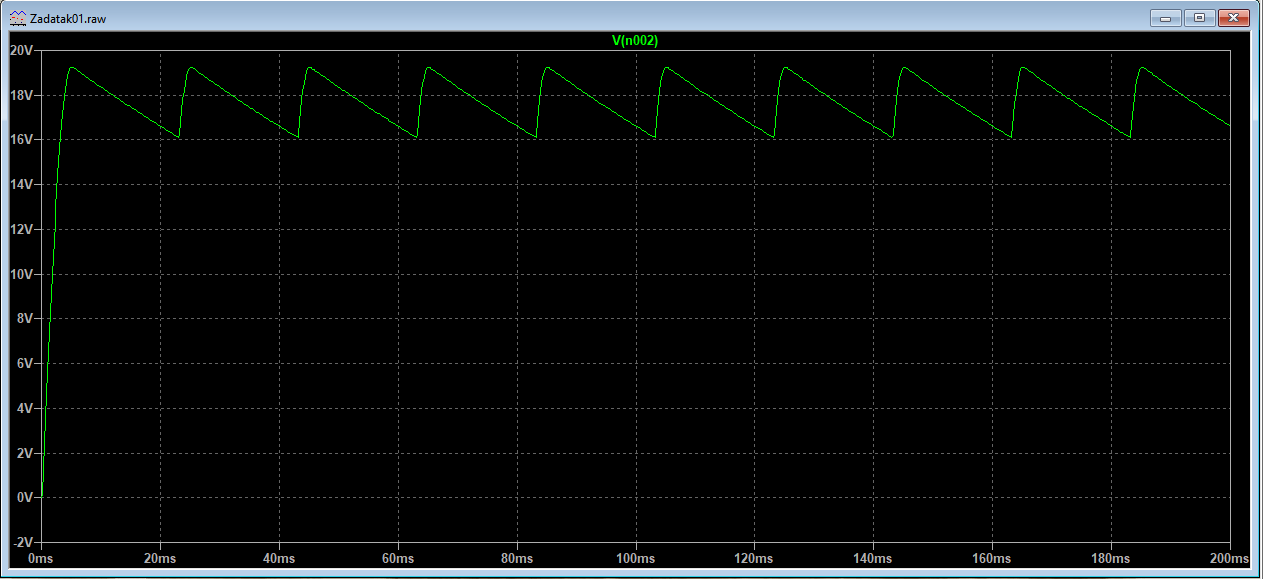
\includegraphics[width=\textwidth]{Zadatak01_1.png}
        \caption[]{Napon potrošača u vremenskom domenu}
    \end{center}
\end{figure}

\begin{figure}[H]
    \begin{center}
        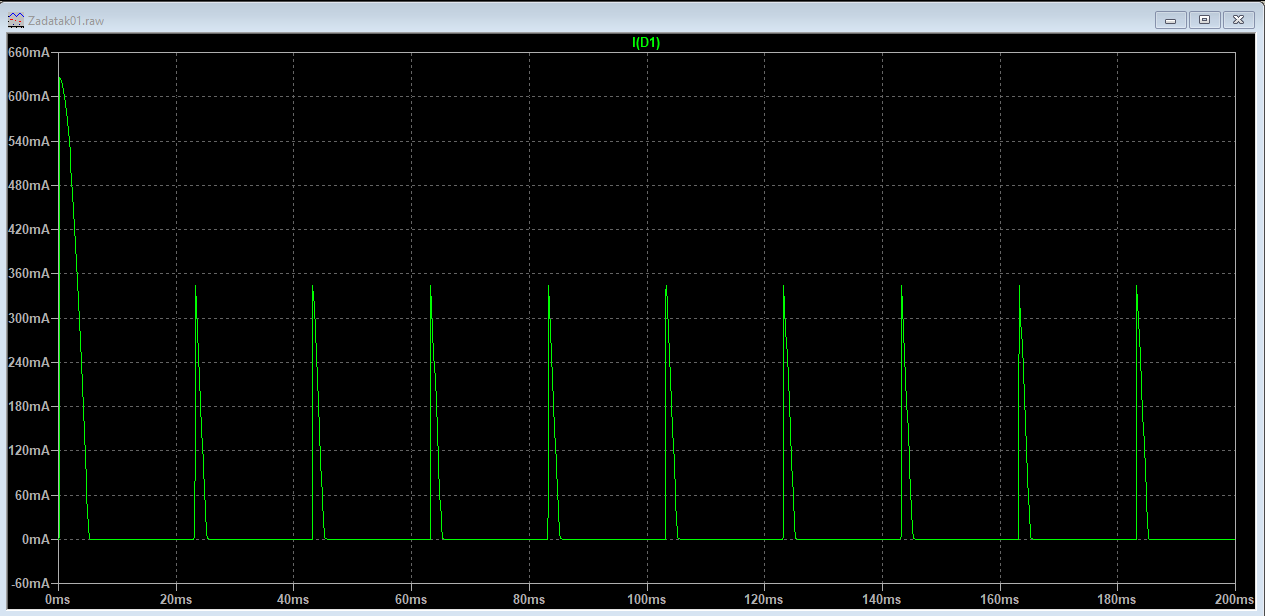
\includegraphics[width=\textwidth]{Zadatak01_2.png}
        \caption[]{Struja naponskog generatora u vremenskom domenu}
    \end{center}
\end{figure}

\begin{figure}[H]
    \begin{center}
        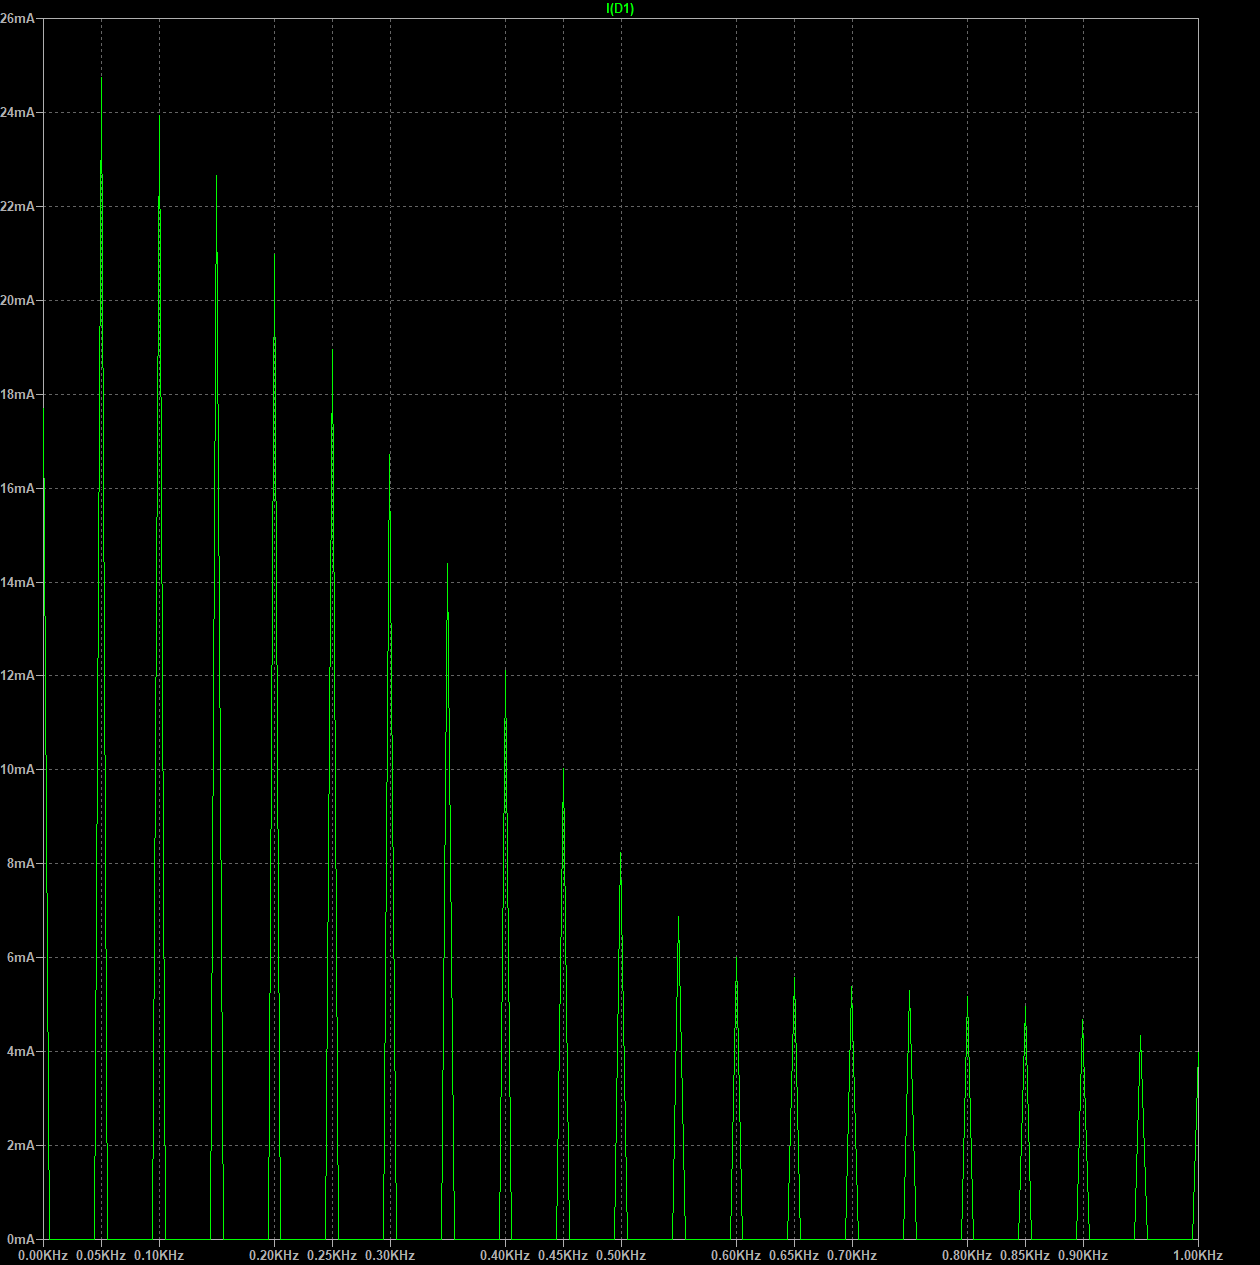
\includegraphics[width=\textwidth]{Zadatak01_3.png}
        \caption[]{Struja naponskog generatora u frekvencijskom domenu}
    \end{center}
\end{figure}

Pitanje: \emph{Na kojim učestanostima se generišu harmonici struje mreže za napajanje?\\}

Na osnovu \emph{slike 3}, to su učestanosti koje zadovoljavaju formulu:
\begin{align}
    f=k*50Hz, k\epsilon N 
\end{align}


\section*{Zadatak 2}

\begin{figure}[H]
    \begin{center}
        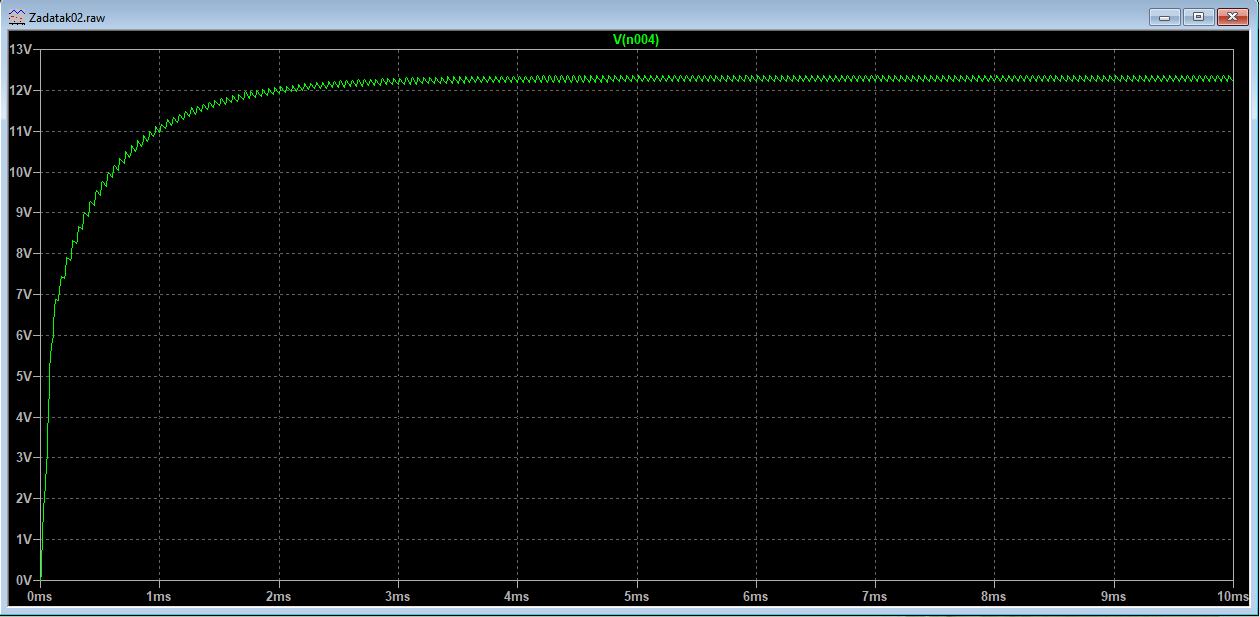
\includegraphics[width=\textwidth]{Zadatak02_1.png}
        \caption[]{Napon potrošača u vremenskom domenu}
    \end{center}
\end{figure}

\begin{figure}[H]
    \begin{center}
        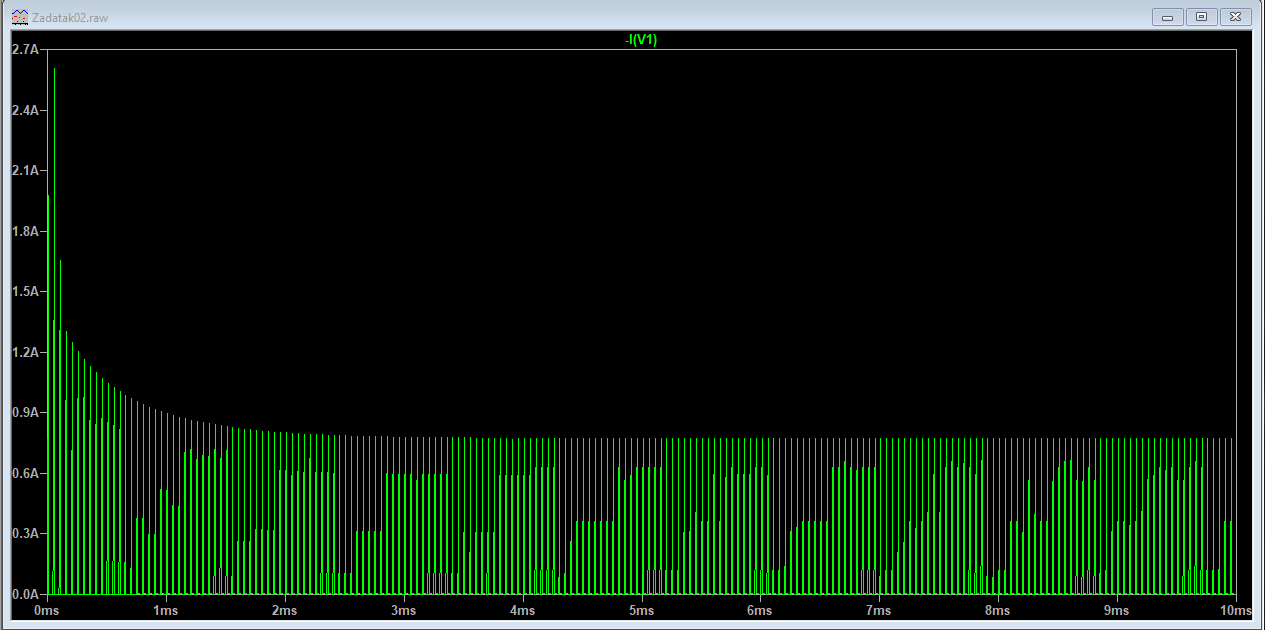
\includegraphics[width=\textwidth]{Zadatak02_2.png}
        \caption[]{Struja naponskog generatora u vremenskom domenu}
    \end{center}
\end{figure}

\begin{figure}[H]
    \begin{center}
        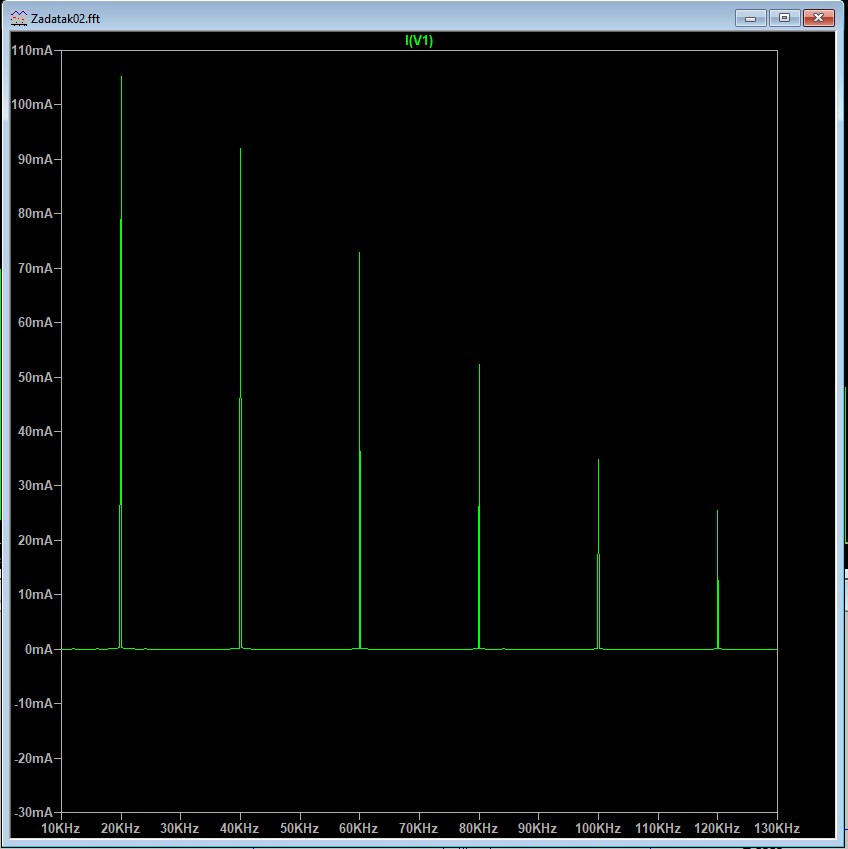
\includegraphics[width=\textwidth]{Zadatak02_3.png}
        \caption[]{Spektar struje naponskog generatora}
    \end{center}
\end{figure}

Pitanje: \emph{Na kojim učestanostima se generišu smetnje ka mreži za napajanje?\\}

Na osnovu \emph{slike 6}, to su učestanosti koje zadovoljavaju formulu:
\begin{align}
    f=k*20kHz, k\epsilon N
\end{align}

\section*{Zadatak 3}

\begin{figure}[H]
    \begin{center}
        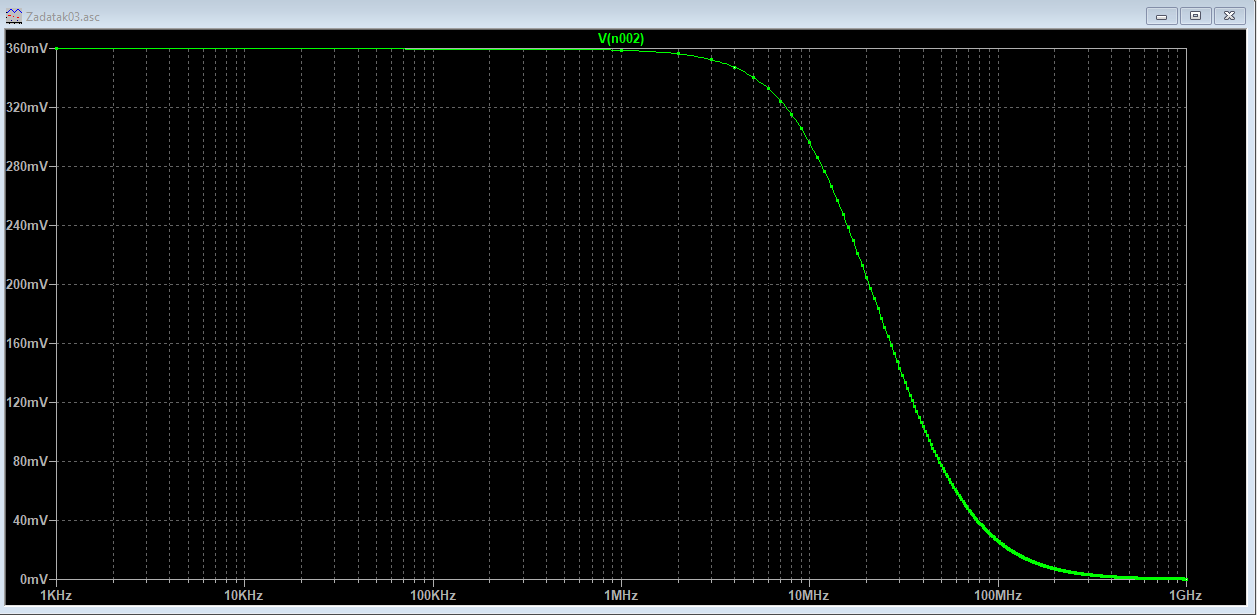
\includegraphics[width=\textwidth]{Zadatak03_1.png}
        \caption[]{Napon na izlazu filtra u frekvencijskom opsegu od \emph{1kHz} do \emph{1GHz}}
    \end{center}
\end{figure}

\begin{figure}[H]
    \begin{center}
        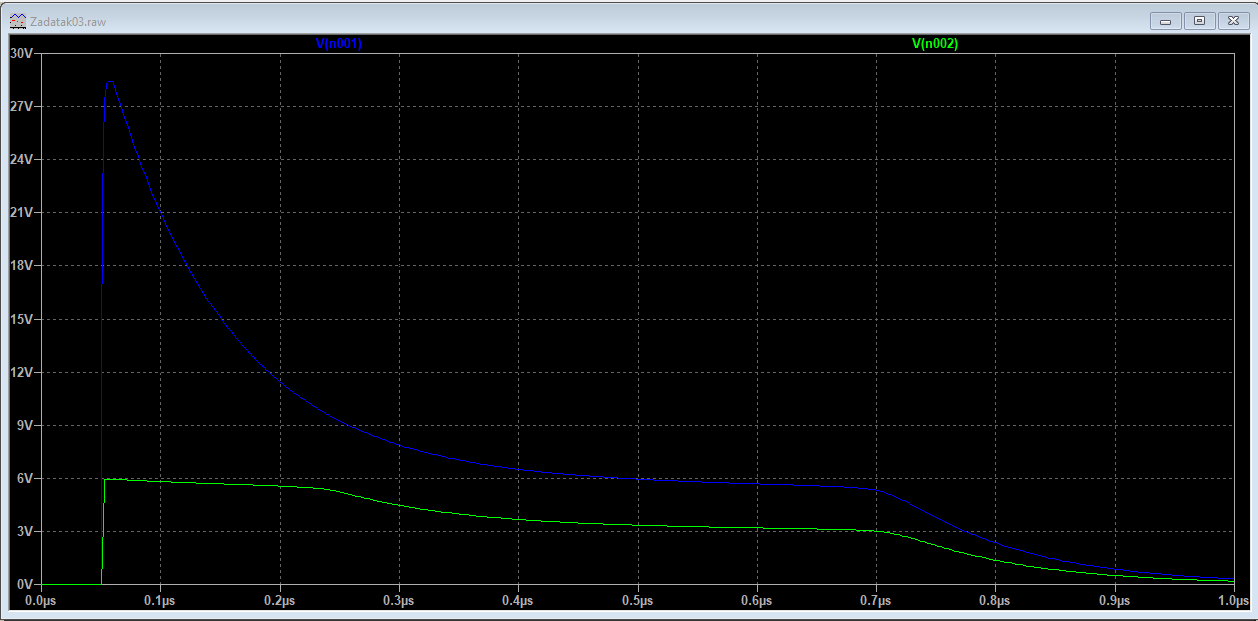
\includegraphics[width=\textwidth]{Zadatak03_2.png}
        \caption[]{Napon na ulazu \emph{(plavo)} i izlazu \emph{(zeleno)} filtra u intervalu \emph{$0 \le t \le 10\mu s$}}
    \end{center}
\end{figure}

Pitanje:
\emph{Ukoliko se zahteva da napon u slučaju elektrostatičkog pražnjenja
 ne sme preći 10V, da li se dodavanjem ovog filtra postiže zaštita potrošača $R=50\Omega$?}\\

Kao sto možemo da vidimo na slici 8, čak i u slučaju simuliranog pražnjenja s pikom od 15kV, vrenosti na potrošaču ne prelaze 6V.

\end{document}